\documentclass[12pt,a4paper]{article}
\usepackage{nopageno}
\usepackage[polish]{babel}
\usepackage[T1]{fontenc}
\usepackage[utf8]{inputenc}
\usepackage{amsmath,amsfonts}
\usepackage{titling}
\usepackage{mathtools}
\usepackage[margin=0.6in]{geometry} 
\usepackage{graphicx}
\usepackage{tikz}

\title{AiSD Zadanie 5 L2}
\author{Cezary Świtała}

\begin{document}

\noindent
\textbf{Zadanie 5} Udowodnij poprawność algorytmu Boruvki (Sollina).

Przedstawmy ideę algorytmu Boruvki:

\begin{enumerate}
	\item Tworzymy graf pomocniczy z samych superwierzchołków (na początku są to po prostu wierzchołki).
	\item Dla każdego superwierzchołka dodajemy najlżejszą incydentną krawędź do grafu pomocniczego.
	\item Superwierzchołki, między którymi istnieje teraz ścieżka łączymy w jeden superwierzchołek.
	\item Powtarzamy, aż nie otrzymamy pojedynczego superwierzchołka.
\end{enumerate}
Algorytm ma działać przy przy założeniu, że każda para krawędzi w grafie ma różną długość.
\vskip 0.5cm
\noindent
Udowodnimy, że algorytm jest poprawny.

\noindent
\textbf{Lemat 1.} \emph{Algorytm znajduje drzewo rozpinające}. Wystarczy, że pokażemy, że w każdej iteracji superwierzchołki są drzewami, wtedy w szczególności po zakończeniu algorytmu nasz ostatni superwierzchołek będzie drzewem zawierającym wszystkie wierzchołki, czyli drzewem rozpinającym.

\vskip 0.5cm
\noindent
\textbf{Lemat 1.1} \emph{Algorytm nie tworzy cykli.} Wystarczy pokazać, że w dowolnym kroku, żaden superwierzchołek nie ma cyklu.

Zaczynamy od grafu, w którym są superwierzchołki są pojedynczymi wierzchołkami, są to oczywiście grafy bez cyklu.

Załóżmy nie wprost, że w którejś iteracji algorytmu powstał cykl w jakimś superwierzchołku \(S\). Rozważymy tą sytuację.

\begin{itemize}
	\item Powiedzmy, że \(S\) powstał z superwierzchołków z poprzedniego kroku \(S_1\) i \(S_2\) 
	i krawędzi do nich dołączonych -- odpowiednio -- \(e_1\) i \(e_2\). Skoro \(e_1\) 
	zostało dołączone do 
	\(S_1\), a	 nie \( e_2 \) to  \( c(e_1) < c(e_2) \), ale skoro \(e_2\) została dołączona do 
	\(S_2\), zamiast \(e_1\), to \( c(e_2) < c(e_1) \) i otrzymujemy sprzeczność.
	\item Rozumowanie to można uogólnić. Powiedzmy, że \(S\) powstał z trzech lub więcej
	superwierzchołków \(S_1, S_2, S_3, ... \) z poprzedniego
	kroku oraz krawędzi \( e_1, e_2, e_3, ... \) do nich przyłączonych. W \(S\) Pojawił się jakiś 
	cykl \(C\), który musiał być złożony z jakichś superwierzchołków \(S_1, S_2, S_3, ...., S_l\) i 
	krawędzi \( e_1, e_2, e_3, ..., e_l \) położonych na przemian.
	\begin{center}
		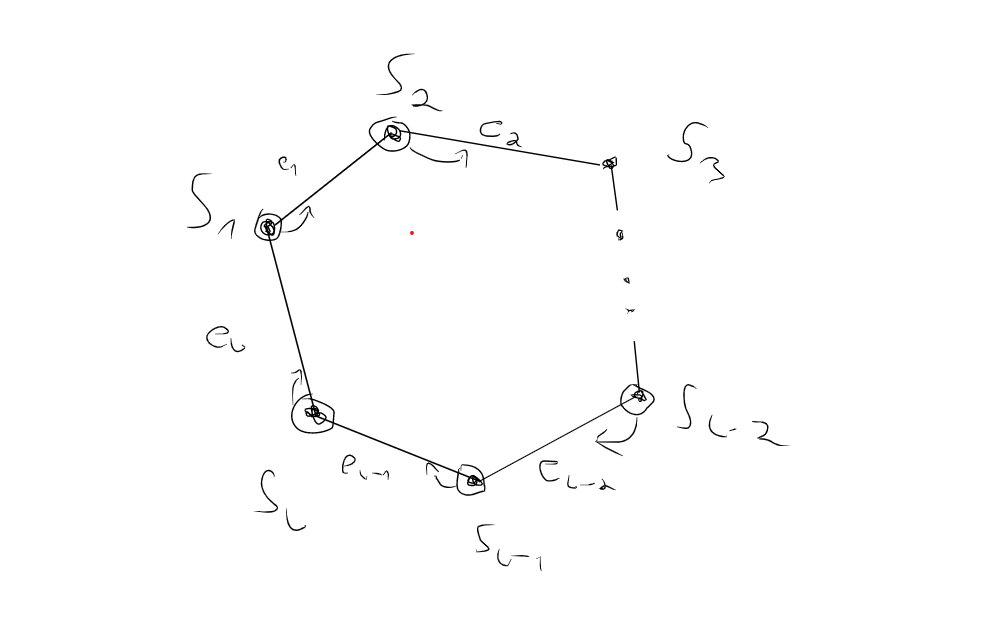
\includegraphics[scale=0.5]{boruvka} 
	\end{center}
	Jak widać na powyższym rysunku skoro \( e_2 \) zostało dołączone do \(S_2\) zamiast \(e_1\) to 
	\(c(e_1) > c(e_2)\). Kontynuując to rozumowanie dla każdego wierzchołka otrzymujemy nierówność
	\[ c(e_1) > c(e_2) > ... > c(e_{l-1}) > c(e_l) > c(e_1) \]
	Z której wynikałoby, że \( c(e_1) > c(e_1) \), więc mamy sprzeczność.
\end{itemize}

\vskip 0.5cm
\noindent
\textbf{Lemat 1.2} \emph{W każdym kroku algorytmu superwierzchołki są spójne.} Zaczynamy od pojedynczych wierzchołków, które są spójne. Później tworzymy kolejne łącząc krawędziami grafy spójne z czego na pewno otrzymamy graf spójny.

\vskip 0.5cm
\noindent
Z \textbf{lematu 1.1} i \textbf{lematu 1.2} wynika, że w każdym kroku superwierzchołki są spójnymi acyklicznymi grafami, czyli drzewami, a skoro ostatecznie otrzymamy jeden superwierzchołek, który zawiera wszystkie wierzchołki, to będzie on drzewem rozpinającym, co dowodzi prawdziwości \textbf{lematu 1}.

\vskip 0.5cm
\noindent
\textbf{Chad lemat 2.} \emph{Wynikowy superwierzchołek jest MST grafu.} Pokażemy indukcyjnie, że w każdej iteracji powstały graf jest podgrafem jakiegoś MST.

\textbf{Podstawa:} W pierwszej iteracji superwierzchołki to po prostu pojedyncze wierzchołki, więc są one podgrafem każdego \textbf{MST}.

\textbf{Krok:} Załóżmy, że graf \(T_k\) był podgrafem jakiegoś \textbf{MST}, nazwijmy je \(M\). Oraz załóżmy nie wprost, że graf powstały w kolejnym kroku -- \(T_{k+1}\) nie jest podgrafem \(M\). Wtedy istnieje krawędź \(e \in T_{k+1}\) i \(e \notin M\), która została dodana w obecnym kroku. Dodajmy ją do \(M\). Wtedy mamy w nim cykl. Skoro \(e\) łączyła jakieś superwierzchołki \(S_i, S_j\), to znajdziemy inną krawędź \(f\in M\), która łączy wierzchołki z superwierzchołka \(S_i\) z innymi, ale skoro nie została dołaczona do grafu \(T_{k+1}\) to z działania algorytmu wnioskujemy \(w(f) > w(e)\). Możemy teraz stworzyć nowe drzewo \(N = M \setminus \{f\} \cup \{e\}\), które ma mniejszą wagę niż \(M\), więc sprzeczność z tym , że \(M\) było \textbf{MST}.

\end{document}